\documentclass[12pt]{aghdpl}
% \documentclass[en,11pt]{aghdpl}  % praca w języku angielskim

% Lista wszystkich języków stanowiących języki pozycji bibliograficznych użytych w pracy.
% (Zgodnie z zasadami tworzenia bibliografii każda pozycja powinna zostać utworzona zgodnie z zasadami języka, w którym dana publikacja została napisana.)
\usepackage[english,polish]{babel}

% Użyj polskiego łamania wyrazów (zamiast domyślnego angielskiego).
\usepackage{polski}

\usepackage[utf8]{inputenc}

% dodatkowe pakiety

\usepackage{mathtools}
\usepackage{amsfonts}
\usepackage{amsmath}
\usepackage{amsthm}
\usepackage{array}
\usepackage{tabularx}

\newenvironment{conditions}
{\par\vspace{\abovedisplayskip}\noindent
\tabularx{\textwidth}{>{$}l<{$} @{${}={}$} >{\raggedright\arraybackslash}X}}
{\endtabularx\par\vspace{\belowdisplayskip}}


% --- < bibliografia > ---

\usepackage[
backend=biber,
style=numeric,
sorting=none,
%
% Zastosuj styl wpisu bibliograficznego właściwy językowi publikacji. 
language=autobib,
autolang=other,
% Zapisuj datę dostępu do strony WWW w formacie RRRR-MM-DD.
urldate=iso8601,
% Nie dodawaj numerów stron, na których występuje cytowanie.
backref=false,
% Podawaj ISBN.
isbn=true,
% Nie podawaj URL-i, o ile nie jest to konieczne.
url=false,
%
% Ustawienia związane z polskimi normami dla bibliografii.
maxbibnames=3,
]{biblatex}

\usepackage{csquotes}
% Ponieważ `csquotes` nie posiada polskiego stylu, można skorzystać z mocno zbliżonego stylu chorwackiego.
\DeclareQuoteAlias{croatian}{polish}

\addbibresource{bibliografia.bib}

% Nie wyświetlaj wybranych pól.
%\AtEveryBibitem{\clearfield{note}}


% ------------------------
% --- < listingi > ---

% Użyj czcionki kroju Courier.
\usepackage{courier}

\usepackage{listings}
\lstloadlanguages{TeX}

\lstset{
	literate={ą}{{\k{a}}}1
           {ć}{{\'c}}1
           {ę}{{\k{e}}}1
           {ó}{{\'o}}1
           {ń}{{\'n}}1
           {ł}{{\l{}}}1
           {ś}{{\'s}}1
           {ź}{{\'z}}1
           {ż}{{\.z}}1
           {Ą}{{\k{A}}}1
           {Ć}{{\'C}}1
           {Ę}{{\k{E}}}1
           {Ó}{{\'O}}1
           {Ń}{{\'N}}1
           {Ł}{{\L{}}}1
           {Ś}{{\'S}}1
           {Ź}{{\'Z}}1
           {Ż}{{\.Z}}1,
	basicstyle=\footnotesize\ttfamily,
}

% ------------------------

\AtBeginDocument{
	\renewcommand{\tablename}{Tabela}
	\renewcommand{\figurename}{Rys.}
}

% ------------------------
% --- < tabele > ---

\usepackage{array}
\usepackage{tabularx}
\usepackage{multirow}
\usepackage{booktabs}
\usepackage{makecell}
\usepackage[flushleft]{threeparttable}

% defines the X column to use m (\parbox[c]) instead of p (`parbox[t]`)
\newcolumntype{C}[1]{>{\hsize=#1\hsize\centering\arraybackslash}X}


%---------------------------------------------------------------------------

\author{Tomasz Kańka}
\shortauthor{T. Kańka}

%\titlePL{Przygotowanie bardzo długiej i pasjonującej pracy dyplomowej w~systemie~\LaTeX}
%\titleEN{Preparation of a very long and fascinating bachelor or master thesis in \LaTeX}

\titlePL{Sprzętowo-programowy system wizyjny do detekcji obiektów zwykorzystaniem termowizji}
\titleEN{Hardware-software vision system for object detection with the use of thermovision.}


\shorttitlePL{Sprzętowo-programowy system wizyjny do detekcji obiektów z wykorzystaniem termowizji} % skrócona wersja tytułu jeśli jest bardzo długi
\shorttitleEN{Hardware-software vision system for object detection with the use of thermovision.}

\thesistype{Praca dyplomowa magisterska}
%\thesistype{Master of Science Thesis}

\supervisor{dr inż. Tomasz Kryjak}
%\supervisor{Marcin Szpyrka PhD, DSc}

\degreeprogramme{Automatyka i Robotyka}
%\degreeprogramme{Computer Science}

\date{2017}

\department{Katedra automatyki i inżynierii biomedycznej}
%\department{Department of Applied Computer Science}

\faculty{Wydział Elektrotechniki, Automatyki,\protect\\[-1mm] Informatyki i Inżynierii Biomedycznej}
%\faculty{Faculty of Electrical Engineering, Automatics, Computer Science and Biomedical Engineering}

\acknowledgements{Serdecznie dziękuję \dots tu ciąg dalszych podziękowań np. dla promotora, żony, sąsiada itp.}


\setlength{\cftsecnumwidth}{10mm}

%---------------------------------------------------------------------------
\setcounter{secnumdepth}{4}

\begin{document}

\titlepages

% Ponowne zdefiniowanie stylu `plain`, aby usunąć numer strony z pierwszej strony spisu treści i poszczególnych rozdziałów.
\fancypagestyle{plain}
{
	% Usuń nagłówek i stopkę
	\fancyhf{}
	% Usuń linie.
	\renewcommand{\headrulewidth}{0pt}
	\renewcommand{\footrulewidth}{0pt}
}

\setcounter{tocdepth}{2}
\tableofcontents
\clearpage

\chapter{Wstęp}
\label{cha:wstep}

Cyfrowa analiza obrazów znalazła szerokie zastosowanie w wielu dziedzinach życia. Umożliwia automatyczne uzyskanie istotnych dla podmiotu informacji na podstawie obrazu bez konieczności angażowania człowieka. Niektóre informacje zawarte w obrazie nie są dobrze dostrzegane przez ludzką percepcję np. kolor jest bardzo subiektywnym parametrem dla różnych ludzi. Przez ostanie kilkadziesiąt lat opracowano tysiące różnych technik i algorytmów wyspecjalizowanych do określonych zadań np. kontrola jakości i przebiegu procesu przemysłowego, kontrola dostępu poprzez rozpoznawanie twarzy w iPhone, optymalizacja ruchu na skrzyżowaniach, bezobsługowe systemy bezpieczeństwa i monitoringu, autonomiczne pojazdy, leśne fotopułapki do badania zachowań i migracji zwierząt itp. Dzisiejsza technologia nie ogranicza nas tylko do stosowania spektrum wiatła widzialnego ludzkim okiem. Kamery na podczerwień stają się coraz tańsze i coraz bardziej popularne. Dostarczają nam informacje o temperaturze obserwowanych obiektów i jest coraz chętniej wykorzystywane w wielu różnych dziedzinach np. weterynarii do określenia miejsc urazów zwierząt, kontroli jakości artykułów spożywczych, analiza strat cieplnych w budynkach, detekcji gazów, systemy wspomagania kierowcy\cite{gade2014thermal}. 

Większość systemów wizyjnych służących do rozpoznawania przechodniów są oparte o analizę obrazów z zakresu światła widzialnego, bądź podczerwieni. W przypadku światła widzialnego można uzyskać bardzo dobre wyniki pod warunkiem że wyszukiwane obiekty są dobrze oświetlone i wyróżniają się swoim kolorem od tła. Podczerwień, a szczególnie termowizja, umożliwia detekcję w warunkach nocnych i ograniczonej widoczności. Oba podejścia mają swoje wady i zalety które wzajemnie się uzupełniają np. duże nasłonecznienia powoduje że tło termiczne staje się dużo wyższe co utrudnia wyodrębnienie pieszego, natomiast daje idealne warunki do uzyskania dobrej jakości obrazu w zakresie widzialnym \cite{lee2015robust}. Połączenie tych dwóch obrazów daje możliwość uzyskania jeszcze lepszych metod rozpoznawania ludzi. W pracy \cite{st2007combination} autorzy nazywają ten rozszerzony format jako RGBT (“Red-Green-Blue-Thermal”), natomiast inna praca jako analizę wielospektralną (Multispectral) \cite{hwang2015multispectral}, albo po prostu jako połączony obraz z kamery termowizyjnej i zwykłej\cite{lee2015robust}. 

Skuteczna detekcja obiektów jest często okupiona dużym zapotrzebowaniem na zasoby obliczeniowe. W wielu przypadkach nie da się uzyskać satysfakcjonującej wydajności by można było uznać  system za działający w czasie rzeczywistym wykorzystując jedynie komputer. Daję to pole do popisu dla układów rekonfigurowalnych które mają możliwość dużego zrównolegnienia obliczeń. Układy FPGA (ang. field-programmable gate array) znalazły już zastosowani w wielu systemach wizyjnych wykonując różnego rodzaju niskopoziomowe operacje kontekstowe, zamiany przestrzeni barw czy też binearyzacji nawet w czasie jednego cyklu zegara. Dodatkową zaletą układów FPGA jest mały pobór mocy co czyni je niezwykle atrakcyjna dla mobilnych aplikacji takich jak drony czy czujniki środowiskowe \cite{garcia2014survey}. 

Niniejsza praca jest kontynuacją pracy inżynierskiej autora.

\section{Cel pracy}


Celem pracy jest realizacja wbudowanego systemu wizyjnego do detekcji wybranych obiektów (np. ludzi) na podstawie obrazu z kamery termowizyjnej. Zakłada się, że jako platforma obliczeniowa zostanie użyty układ heterogeniczny (np. Zynq firmy Xilinx), który umożliwia realizację sprzętowo-programową algorytmów.

\section{Struktura pracy}

W pierwszej części została opisana budowa cyfrowego systemu wizyjnego z wykorzystaniem połączonych obrazów RGB oraz IR. Zawiera teorię tworzącą podstawę dla następnych rozdziałów oraz kilka przykładów już zrealizowanych systemów. W następnym rozdziale została podana specyfikacja techniczna zastosowanych urządzeń oraz technologii. W rozdziale czwartym opisano realizacja autorskiego systemu detekcji ludzi. Prace zakończono podaniem osiągniętych wyników i wnioskami.
\chapter{Cyfrowy system wizyjny}
\label{cha:csw}

\section{Podczerwień}

Jako podczerwień określa się promieniowanie elektromagnetyczne w zakresie długości fali od  0,75 $\mu m$ do 1000~$\mu m$. Ciało które ma temperaturę powyżej zera absolutnego emituje swoją powierzchnią promieniowanie. Im większa jest temperatura ciała tym większa jest jego emisja. Dla każdej temperatury danego ciała istnieje charakterystyczna długość fali o najwyższej wartości mocy promieniowania. Im wyższa temperatura tym ta częstotliwość przesuwa się w zakres fal widzialnych. Można to zaobserwować gdy stal osiąga wysoką temperaturę powodując tym emisję światła. Ciało doskonale czarne całkowicie pochłania padające na nie promieniowanie, oraz emituję promieniowanie ściśle związane z jego temperaturą. Wykres na rysunku \ref{fig:perfect_black}  przedstawia tą charakterystykę. Promieniowanie podczerwone jest częściowo pochłaniane przez atmosferę ziemską . Na rysunku  \ref{fig:atmosfera_int} przedstawiono transmisyjność atmosfery. W aparaturze obrazującej w podczerwieni wykorzystuję się dwa zakresy przy których transmisyjność jest największa:  3 -- 5 $\mu m$ (MIWR, ang. \textit{mid wave infrared} - podczerwień fal średnich) oraz  8 -- 14 $\mu m$ (LWIR , ang. \textit{long wave infrared} - podczeriwń fal długich)\cite{niklaus2007mems}.

\begin{figure}
\centering
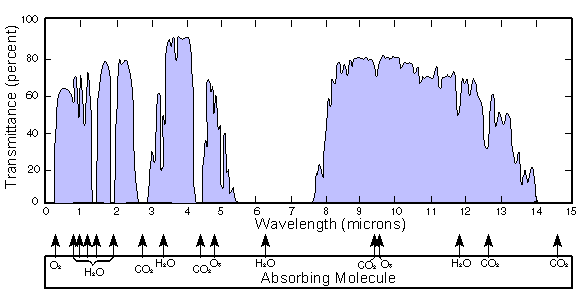
\includegraphics[width=0.8\linewidth]{images/Atmosfaerisk_spredning}
\caption[Wykres transmisyjności atmosfery dla promieniowania podczerwonego ]{Wykres transmisyjności atmosfery dla promieniowania podczerwonego \cite{wiki:infrared}.}
\label{fig:perfect_black}
\end{figure}

\begin{figure}
\centering
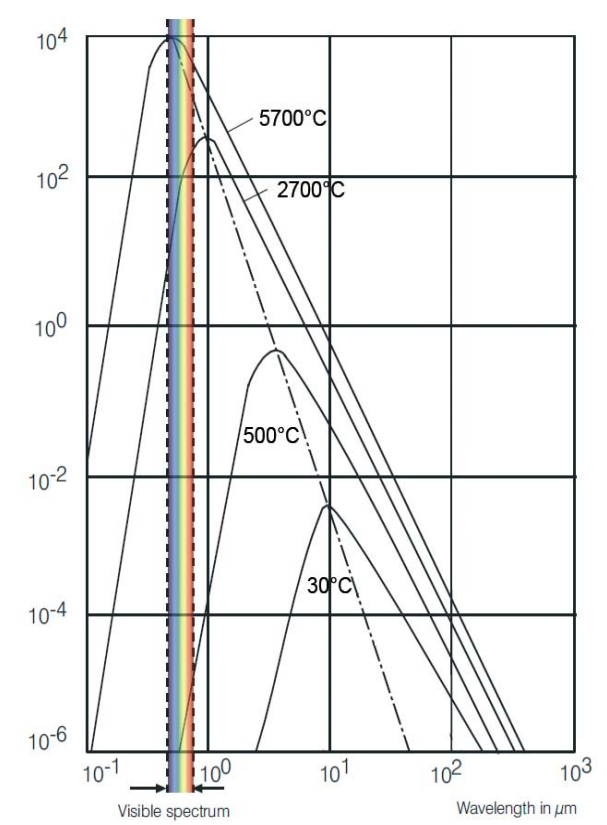
\includegraphics[width=0.4\linewidth]{images/perfect_black_emi}
\caption[Emisyjność ciała idealnie czarnego]{Emisyjność ciała idealnie czarnego.}
\label{fig:atmosfera_int}
\end{figure}

\section{Metody akwizycja obrazu i kalibracja}

Większość implementacji wykorzystuje układ dwóch równoległych do siebie kamer. Do połączenia obrazów należy zastosować algorytm wyrównujący oba obrazy. Kalibrację wykonuję się specjalnymi  planszami które pozwalają określić położenie punktów kalibracyjnych w obu rejestrowanych zakresach. Plansze mogą być aktywne (posiadają własne źródło ciepła) albo pasywne (przesłaniają obce źródło ciepła). W tym układzie występuję również zjawisko paralaksy które powiększa się wraz z wzrostem odległości obiektu od punktu kalibracji. W pracy  \cite{hwang2015multispectral} autorzy zastosowali zwierciadło półprzezroczyste wykonane z wafla krzemowego pokrytego cynkiem do rozdzielenia obrazu co wyeliminowało wady układu równoległego.

\begin{figure}[h]
	\centering
	\begin{subfigure}{0.45\textwidth}
		\centering
		 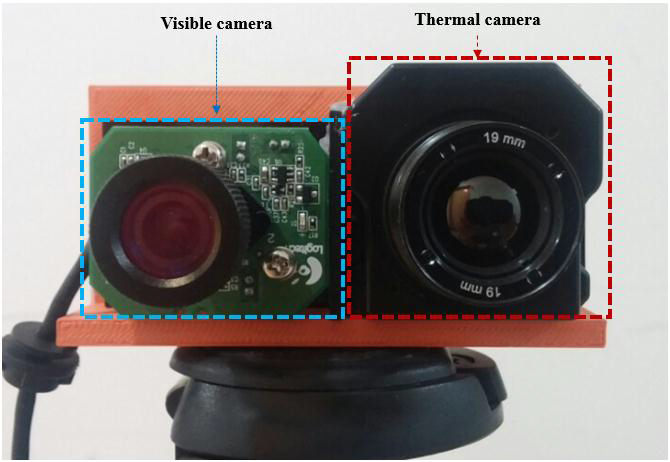
\includegraphics[width=1\textwidth]{images/dual-camera}
		\subcaption{\label{dual_camera}}
	\end{subfigure}
	\begin{subfigure}{0.45\textwidth}
		\centering
		 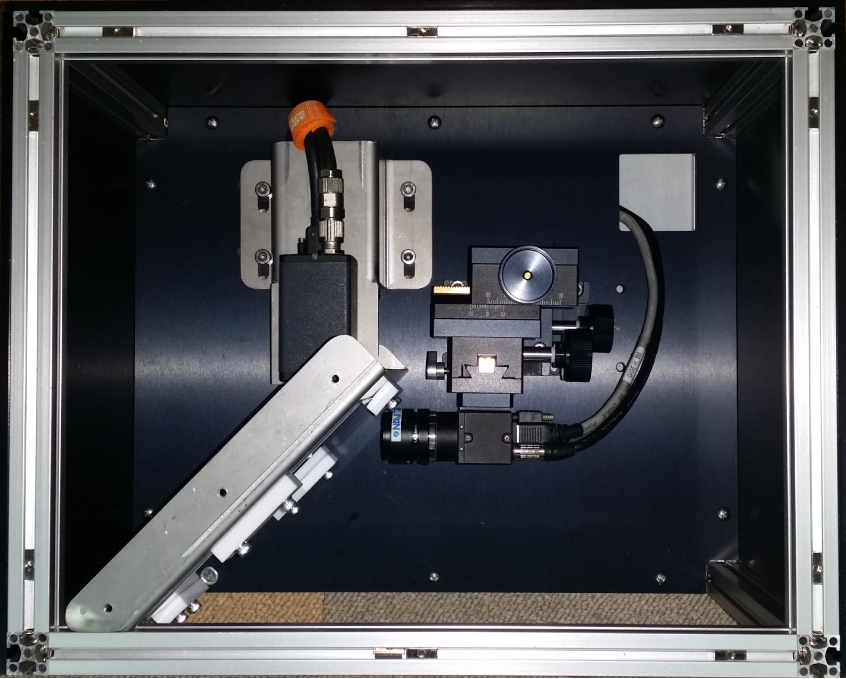
\includegraphics[width=1\textwidth]{images/multispectral}
		\subcaption{\label{multispectral}}
	\end{subfigure}
	
	\caption{\label{fig:cameras_systems}Sposoby akwizycji obrazów:  \protect\subref{dual_camera} dwie kamery równolegle \cite{lee2015robust}, \protect\subref{multispectral} z wykorzystaniem zwierciadła półprzezroczystego \cite{hwang2015multispectral}.}
\end{figure}

\section{Model geometryczny}

Do opisu matematycznego systemu wykorzystuje się model kamery otworowej. Dzięki niej można opisać relację między trójwymiarową przestrzenią a dwuwymiarowym obrazem za pomocą projekcji perspektywicznych. Nie stanowi on najdokładniejszego opisu matematycznego kamery, nie ma uwzględnionych w nim zakłóceń soczewkowych, ale jest wystarczające dobre dla niektórych zastosowań. Składa się ona z 2 zestawów parametrów: zewnętrznych oraz wewnętrznych. Parametry zewnętrzne definiują lokację kamery względem zewnętrznego układu współrzędnych. Są reprezentowane przez wektor translacji \(T\) między układem związanym z kamerą \( \left (  X_{c},Y_{c},Z_{c}\right ) \)
 a zewnętrznym \(\left (  X,Y,Z\right )\). Drugim parametrem jest macierz rotacji \( R \)( między osiami tych dwóch układów.
Punkt \(P = \left [ X,Y,Z \right ]^T \) będący w zewnętrznym układzie współrzędnym ma swój odpowiednik w układzie wewnętrznym który można określić zależnością 

\begin{equation}
P_{c} = RP+T
\end{equation}

Właściwości optyczne kamery można przedstawić w postaci macierzy kamery.

\begin{equation}
K = \begin{bmatrix}
f_x & 0 & x_0 \\ 
0 & f_y & y_0\\ 
0 &0  & 1
\end{bmatrix}
\end{equation}
gdzie:
\begin{conditions}
f_{x}, f_{y} & ogniskowa kamery wyrażona w liczbie pikseli, \\
x_{0},y_{0} & współrzęne punktu głównego. 
\end{conditions}

Macierz K określa związek między między znormalizowanymi współrzędnymi w układzie odniesienia kamery, danych wzorem \(x_n = \frac{X_c}{Z_c}, y_n = \frac{Y_c}{Z_c}\), a odpowiadającym im wspórzędnymi punktów na obrazie \(u,v\):

\begin{equation}
\begin{bmatrix}
u \\
v \\
1
\end{bmatrix} = K \begin{bmatrix}
x_n \\
y_n \\
1
\end{bmatrix}
\end{equation}
W pracy \cite{rangel20143d} autorzy sprawdzili kila różnych plansz kalibracyjnych i najlepsza okazała się z kartonu... TO DO: dopisać.


\section{Algorytmy detekcji pieszych}

W cyfrowej analizie obrazu rozpoznawanie pieszych jest jedną z najbardziej aktywnych i rozwijanych dziedzin. W przeciągu kilkudziesięciu lat powstało ponad tysiąc artykułów poruszających to zagadnienie \cite{zhang2015filtered} i wiele różnych metod zostało już opracowanych. Większość metod opiera się o analizę obrazu tylko w jednym spektrum: widzialnym albo podczerwieni. Praca \cite{hwang2015multispectral} pokazała że połączenie obu obrazów może dać lepsze wyniki. Podobnie w \cite{gonzalez2016pedestrian} ustalono że analiza multispektralna jest skuteczniejsza w dzień niż w nocy (o około 5\% AMR (ang. avrange miss rate).   W artykule \cite{benenson2014ten} autorzy podsumowują osiągnięcia w dziedzinie detekcji pieszych w latach 2004 – 2014 wyróżniono ponad 40 różnych podejść do problemu. Artykuł jest oparty o bazę danych Caltech-USA która oferuje obrazy w kolorze. Jednym z wniosków jest że przez ostanie dziesięć lat największy postęp został osiągnięty głównie dzięki dopracowaniu cech jakie są wyodrębniane z obrazu niż ulepszanie klasyfikatora. Dodatkowo autorzy połączyli cechy dające najlepsze wyniki i stworzyli własną metodę która uzyska 12\% zysk AMR względem  najlepszej badanej wcześniej metody.

Dla typowego algorytmu detekcji pieszych można wyróżnić trzy podstawowe etapy:

\subsection{Ustalenie regionu zainteresowań} 
Jest to obszar zwany ROI(ang. Region of interest) w którym potencjalnie mogą znajdować się przechodnie. Wiele podejść uznaje cały obraz jako ROI i stosuje okno przesuwne sprawdzając każdy możliwy fragment obrazu. Jeżeli obraz jest rejestrowany przez nieruchomą kamerę, ROI można określić poprzez różnicę między zapamiętanym tłem a aktualnym obrazem. Wyodrębnienie ROI jest bardzo istotne w przypadku pracy w czasie rzeczywistym ze względu na ograniczony czas analizy pojedynczego obrazu.

\subsection{Wyodrębnienie cech}
Do najbardziej popularnych cech można zaliczyć:

\begin{enumerate}
\item Histogramy zorientowanych gradientów (HOG) zaproponowany przez N.Dalala i B. Triggs w pracy \cite{dalal2005histograms} stała się jedną z najbardziej popularnych techniką w dziedzinie rozpoznawania ludzi. Jest cały czas rozwijana i modyfikowana w wielu pracach naukowych. Technika polega na zliczeniu kierunków gradientów, uzyskanych z 2 masek kierunkowych \(\begin{bmatrix}-1 & 0 & 1\end{bmatrix} \) i \( \begin{bmatrix}-1 & 0 & 1 \end{bmatrix}^T\), w komórkach o określonych wymiarach. Komórki te są organizowane w bloki w obrębie których następuję normalizacja. Wektorem cech jest połączony wszystkich histogramów z wszystkich bloków w jeden wektor.

\item Lokalne wzorce binarne LBP (ang. Local Binary Paterns).  Oryginalnie przeznaczone do opisu tekstur. Obraz zostaje podzielony na bloki. Następnie każdego piksela w bloku zostaje przypisany wzorzec binarny na podstawie wartości pikseli w jego sąsiedztwie. Jeżeli wartość sąsiadującego piksela jest większa od centralnego to przyjmuje on wartość 1. Następnie zostaje obliczony histogram dla każdego bloku. Histogramy z wszystkich bloków wchodzących w skład obrazu tworzą wektor cech \cite{ojala2002multiresolution}.

\item Falki Haara.
Określają różnicę w kontraście między dwoma przylegającymi prostokątnymi obszarami. Są łatwe do skalowania i nie wymagają dużych nakładów obliczeniowych.

\item Kolor. W analizie obrazo wykorzystuje różne przestrzenie barw np. RGB, HSV oraz LUV. 

\item Lokalne struktury. W odróżnieniu od pojedynczych pikseli można wyznaczyć lokalne struktury o podobnym kolorze. (np. głowa i ręce mają podobne kolory, jednolita koszula, spodnie)


\end{enumerate}

\subsection{Klasyfikator}
Otrzymany wektor cech jest poddany klasyfikacji której wynik decyduje czy obraz zawiera człowieka. W pracy \cite{benenson2014ten} autorzy wyróżnili 3 dominujące rodziny:

\begin{enumerate}
\item Rodzina DPM (ang. Deformable Part Detectors) ??? wykrywacze deformowlnych elementów ???. Technika polega na klasyfikacji poszczególnych elementów człowieka (głowa, tułów, nogi). Następnie  jest analizowany układ tych elementów na obrazie i podjęcie decyzji o obecności człowieka.

\item Deep networks – głębokie sieci neuronowe.

\item Decision forests – ?? lasy decyzyjne ?? zbiór nieskorelowanych drzew decyzyjnych.

\item inne: SVN (ang. support vector machine – maszyna wektorów nośnych), AdaBoost itp.
\end{enumerate}

\section{Przegląd literatury}

\subsection{}

	W pracy \cite{kolzpoz} autorzy opracowali algorytm pozwalający na szybką i efektywną detekcję przechodniów w czasie rzeczywistym . Termowizja pozwala na uzyskanie dobrego kontrastu między poszukiwanym przechodniem a otoczeniem. System dedykowany jest do pracy w nocy kiedy kontrast między człowiekiem pozwala na jednoznaczne ich rozróżnienie. Rozwiązanie bazuję na ulepszonym algorytmie progowania i segmentacji obrazu. Pierwszym etapem jest wyodrębnienie obszarów zainteresowań (ang. ROI). Pozwala to na znaczne ograniczenie obszaru obrazu do analizy. Obraz w odcieniach szarości zostaję poddany binaryzacji z użyciem dwóch progów: mniejszym i większym. Dodatkowo każdy wykryty obszar tworzy dodatkowy ROI przylegający do pierwotnego. Progowanie z pojedynczym progiem jest niewystarczające w wielu wypadach dlatego autorzy zastosowali podwójne progowanie. Pozwala to na detekcję przechodniów w różnych rejonach obrazu o różnym kontraście. Progi zmieniają się wraz z dynamiką obrazu wejściowego. W obrazie termicznym człowieka często występuję obszar o niższej temperaturze w okolicach bioder. Skutkuje to przerwą w zbinearyzowanym obiekcie i błędną klasyfikację np.: samych nóg. Autorzy opracowali technikę polegającą na powiększeniu obszaru. Łączy ona dwie połówki człowieka jeżeli posiadaj wspólne współrzędne wzdłuż pionowej osi tworząc nowy obszar. Ostatecznie obie grupy obszarów zainteresowania uzyskanych z obu progowań zostają połączone. 

	Następnym krokiem jest filtracja wyników. Ma na celu zredukowanie ilości obszarów do końcowej analizy. Autorzy zastosowali filtrację opierającą się na proporcji obszaru zainteresowań. Pozytywnie zakwalifikowane zostały tylko obszary o odpowiednich proporcja wysokości do szerokości (1:1.3 do 1:4). Z racji że badany obraz pochodzi z kamery zamontowanej na stałe na samochodzie autorzy wykorzystali filtrację perspektywiczną. W większej odległości na horyzoncie obiekty są mniejsze. Zakłada ona że w określonych obszarach obrazu istnieje maksymalna możliwa wysokość kandydata. Filtracja jednorodnych regionów pozwoliła na odrzucenie obszarów które często występują jako część szerszych obiektów nie mających nic wspólnego z przechodnimi. Autorzy zaproponowali by obliczenie odchylenia standardowego tych obszarów w odcieniach szarości i odrzucenie części która jest poniżej pewnego progu. 

	Ostatnim krokiem algorytmu jest klasyfikacja wytypowanych kandydatów. Autorzy wykorzystują Histogram zorientowanych gradientów jako cechę tworząc wektor 3780 cech które są przetwarzane przez maszynę wektorów nośnych.

	W celu zbadania dokładności algorytmu został przeprowadzony test na zbiorze CVC-14 zawierający obrazy nagrane kamerą FIR podczas nocnego przejazdu samochodem. Testy wykazały że metoda podwójnego progowania daje trzy razy lepsze rezultaty niż przy wykorzystaniu pojedynczego progu. Wraz z zaproponowanymi technikami filtracji zaowocowało bardzo efektywnym mechanizmem segmentacji. Cała procedura detekcji przechodniów osiągnęła wysoki poziom wydajności na poziomie 33 klatek na sekundę przy wykorzystaniu pojedynczego rdzenia CPU.

\subsection{}
„Pedestrian detection using infrared images and histograms of oriented gradients”

W pracy [] autorzy zaproponowali wykorzystanie dwóch kamer termowizyjnych tworząc system stereowizyjny. By wyodrębnić obszary zainteresowania potencjalnie zawierający w sobie przechodnie wyodrębniano piksele o wartościach powyżej kilku różnych progów. Porównując te dwa obrazy można określić pozycję i odległość źródła ciepła od kamery. W obrazie termowizyjnym człowieka można zauważyć że najbardziej ciepłym i odsłoniętym obszarem ciała jest głowa. Wykorzystując ten fakt, oraz informację o odległości od kamery, zostają wytyczone obszary wokół tych pikseli o wielkości zależnej od odległości. Następnie wszystkie wyodrębnione tak obszary zostają przeskalowane do wymiaru 128x64 piksele i poddane klasyfikacji za pomącą kombinacji HOG+SVM. 
W tej pracy autorzy skupili się na optymalnym dobraniem parametrów HOG. Badanie zostały przeprowadzone na bazie obrazów termowizyjnych o wymiarach 128x64. Zestaw zawierał 4400 obrazów: 2200 zawierających przechodnia oraz 2200 nie zawierających. Został wykorzystany następujący zestaw parametrów HOG:
\begin{enumerate}

\item Wielkość komórki:  4x4, 8x8, 16x16,
\item wielkość bloku: 1x1, 2x2, 4x4,
\item nakładanie się bloków: 1, 2,
\item ilość przedziałów histogramu: 4, 8, 16,
\item- metoda dopasowania: ważony lub nie
\item metoda normalizacja bloku: L1, L2, brak
\end{enumerate}
Parametry dla klasyfikatora SVM :
\begin{enumerate}
\item wielkość zestawu do nauki: 10, 100, 1000 obiektów na klasę,
\item waga źle sklasyfikowanych punktów C: 0.01, 1, 100.
\end{enumerate}
Autorzy przeprowadzili po 10 nauczań klasyfikatora dla każdej kombinacji wykorzystując różne kombinacje danych do nauki i testów. Po przeprowadzonych badaniach został wytypowany optymalny zestaw parametrów:
\begin{enumerate}
\item Wielkość komórki: 8x8, 
\item wielkość bloku: 2x2
\item nakładanie się bloków: 1,
\item ilość przedziałów histogramu: 4, 8, 16,
\item metoda dopasowania histogramu: ważona 
\item metoda normalizacja bloku: L2.
\end{enumerate}
Badanie parametrów dla nauczania SVM wynikło że im większy zestaw uczący tym lepszą można uzyskać skuteczność detekcji. Parametr C miał marginalne znaczenie na wyniki.



\chapter{Wykorzystanie FPGA w analizie obrazu}

	Tradycyjne systemy wizyjne zwykle bazują na architekturze sekwencyjnej, po kolejnym przekształceniu obraz jest sukcesywnie poddawany następnym. W aplikacji procesorowej te operacje są wykonywane przez układ arytmetyczno-logiczny w który jest wyposażony. Kolejne kroki algorytmu są kompilowane w ciąg instrukcji dla procesora który oprócz operacji matematycznych dużą część pracy poświęca na pobieranie i dekodowanie rozkazów oraz na pobieranie i zapisywanie danych do pamięci. By taka aplikacja mogła pracować w czasie rzeczywistym cała procedura musi wykonać się szybciej przychodzące dane obrazu co wymusza wysoki taktowanie procesora sięgające GHz. 
	W przypadku podejścia równoległego, implementacja poszczególnych kroków algorytmu odbywa się w osobnych procesach. Jeżeli kolejne kroki algorytmu wymagałyby danych otrzymanych z poprzednich to zysk takiego zabiegu byłby równy zero.  By uzyskać znacznie przyspieszenie algorytm musi mieć możliwość podzielenia na wiele niezależnych części. Maksymalne do uzyskania przyspieszenie jest określone przez prawo Amdahla: 
\begin{equation}
P_w =\frac{1}{ s + \frac{1-s}{n_w}}
\end{equation}
gdzie:
\begin{conditions}
P_{w} &  przyspieszenie algorytmu w systemie wieloprocesorowym, \\
s &  cześć algorytmu niepodlegająca zrównolegleniu (wartość od zera do jeden), \\
n_{w} & liczba elementów obliczeniowych.
\end{conditions}

Teoretycznie jedynym ograniczaniem w możliwości zrównolegnia obliczeń jest ilość zasobów dostępnych, jednak istotnym aspektem jest sposób dostarczania danych do zaimplementowanych w układzie procesorów. Czas i przepustowość jaka jest potrzebna do odczytania i zapisu obrazu po przetworzeniu z i do pamięci jest najczęściej wąskim gardłem systemu wizyjnego. Z tego powodu przetwarzanie obrazu bezpośrednio z sensora w czasie jego akwizycji jest chętnie wykorzystywane gdyż zmniejsza to ilość operacji odczytu i zapisu.  \cite{garcia2014survey}

\section{Podejście sprzętowo - programowe}

W pracy \cite{honegger2014real} autorzy wykorzystali układ FPGA oraz CPU małej mocy do skonstruowania systemu wizyjnego dla robotów. System analizował obraz steroskopowy z dwóch kamer tworząc mapę głębi. Obie kamery są bezpośrednio podpięte do układu FPGA w którym obrazy są przetwarzane. Następnie dwa oryginalne obrazy oraz mapa głębi są przesyłane do CPU za pomocą specjalnej szyny danych. Moduł frame grabbera przechwytywał ten obraz i wykorzystując DMA (ang. Direct Memeory Acces) zapisywał do pamięci systemu. Ten zabieg gwarantował poprawną transmisję obrazu do CPU. Rozdzielczość oraz ilość klatek na sekundę są w pełni elastyczne dzięki czemu CPU dostawało obraz o szerokości trzy raz większej niż oryginalny obraz. Pozwalało to na przesłanie zsynchronizowanego lewego, prawego obrazu i mapy głębi. System pracował w rozdzielczości 752x480 piksle i 60 klatkach na sekundę. Całość systemu wizyjne włącznie z kamerami, układem FPGA, CPU oraz konwerterami napięcia pobierał mniej niż 5W mocy. Całkowita latencja podana przez autorów rozwiązania wynosi około 2ms.

W pracy \cite{piao2016real} autorzy wykorzystali układ SoC (ang. System on Chip) do detekcji pieszych dla zaawansowanego systemu wspomagania kierowcy (ADSA ang. advanced driver assistance system). Głównym wyzwaniem było opracowanie metody która działa w czasie rzeczywistym, ma mały pobór mocy oraz niski koszt wykonania. Większość topowych algorytmów  wymaga znacznych zasobów obliczeniowych więc autorzy dokonali relaksacji problemu poprzez zastosowanie prostszego deskryptora jakim jest LBP oraz SVM jako klasyfikatora. Autorzy zamontowali po każdej stronie pojazdu inteligentną kamerę o 180$^\circ$ horyzontalnym kącie widzenia by jak najlepiej monitorować przestrzeń wokół niego. W kamerach została przeprowadzona wstępna obróbka obrazu (rektyfikacja i skalowanie). Przetworzony obraz z kamer był transmitowany do „Fusion-Box” gdzie odbywała się generacja kandydatów, klasyfikacja, weryfikacja oraz śledzenie. Wyniki były przesyłane do wbudowanego komputera PC. Rozwiązanie nie zostało jeszcze w pełni zaimplementowane ale pierwsze testy dawały obiecujące rezultaty.



\chapter{Wykorzystane zasoby sprzętowe i technologie}
\section{Kamera termowizyjna Lepton}

\begin{figure}[h]
    \centering
    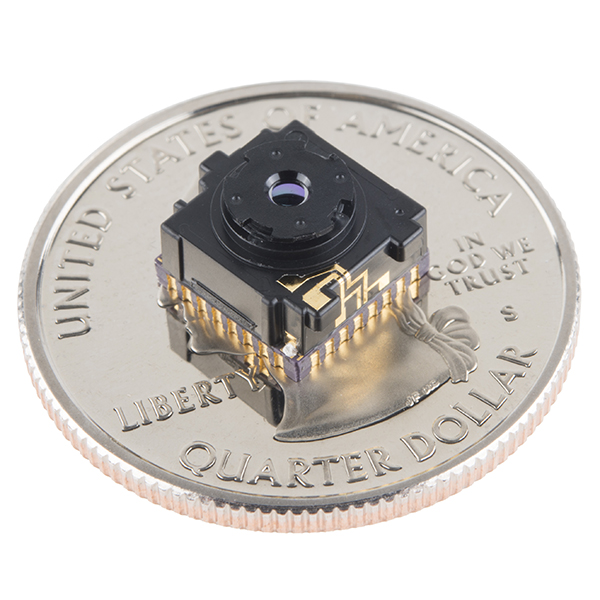
\includegraphics[width=0.6\textwidth]{images/Lepton}
    \caption{Widok poglądowy na kamere Flir Lepton.}
    \label{fig:lepton}
\end{figure}
 
Lepton jest zintegrowaną w pojedynczym układzie kamerą składającą się z soczewki, sensora podczerwieni fal długich (ang. LWIR – long wave infrared) oraz elektroniki sterującej i przetwarzającej sygnał. Checuje siębardzo małymi wymiarami co czyni go idealnym do zastosowań mobilnych. Układ ma możliwość domontowania dodatkowej przesłony która jest wykorzystywana do automatycznej optymalizacji procesu ujednolicania obrazu (kalibracji sensora).
Prosty do integracji z dowolnym mikrokontrolerem dzięki zastosowaniu standardowych protokołów i interfejsów. Lepton po podłączeniu od razu pracuję w domyślnym trybie pracy, który może zostać zmieniony za pomocą CCI (ang. camera control interface – interfejs kontroli kamery).\cite{lepton}
Parametry:
\begin{itemize}
\item Wymiary: 11,8 x 12,7 x 7,2 mm, 
\item Sensor: niechłodzony mikrobolometr VOx (tlenek wanadu),
\item Rejestrowany zakres: fale długie podczerwieni, 8$\mu m$ do 14$\mu m$ ,
\item Wielkość piksela: 17 $\mu$m,
\item Rozdzielczosć: 80x60 pikseli,
\item Ilość klatek na sekundę 8,6,
\item Zakres rejestrowanych temperatur: -10  $^\circ$  C 140  $^\circ$  C (Tryb wysokiego wzmocnienie),
\item korekta niejednorodności matrycy: automatyczna na bazie przepływu optycznego
\item kąt widzenia horyzontalny / diagonalny: 51 $^\circ$ \\ 66 $^\circ$,
\item Głębia ostrości: od 10cm do nieskończoności
\item Format wyjściowy: do wyboru: 14-bit, 8-bit (z AGC (ang. automatic gain control – automatyczna kontrola wzocnienia)) 24-bit rgb (z ACG i koloryzacją).
\item Interfejs video: VoSPI (Video over Serial Peripherial Interface)
\item Interfejs sterujący: CCI (I2C podobny)
\end{itemize}
\section{Zynq-7000}

Rodzina układów Zynq-7000 bazuje na architekturze SoC (ang. System on Chip). Posiadają zintegrowany kompletny system składający podzielonego na dwie części: systemu procesorowego bazującego na procesorze ARM Cortex-A9 (PS ang. Porcessing System) oraz logikę programowalną (PL ang. programable logic) FPGA w jednym układzie scalonym. Na rysunku \ref{fig:zynq7000} przedstawiono schemat architektury. Prócz procesora cześć procesorowa posiada wbudowaną pamięć, kontroler pamięci zewnętrzne oraz szereg interfejsów dla układów peryferyjnych takich jak USB, GigEthernet, CAN, I2C, SPI. W części logiki programowalnej znajdują się bloki logiki konfigurowalnej (CLB ang. configurable logic block), 36Kb bloki pamięci RAM, procesory sygnałowe DSP48, układ JTAG, układy zarządzania zegarami oraz dwa 12-bitowe przetwornik analogowo-cyfrowy.

Komunikacji między częścią procesorową a logiką programowalną odbywa się za pośrednictwem Interfejsu AXI (ang. Advanced Extensible Interface), oraz bezpośrednio wykorzystując porty generalnego przeznaczenia, przerwania, oraz poprzez bezpośredni dostęp do pamięci (DMA ang. Direct Memory Access) 

\begin{figure}[h]
    \centering
    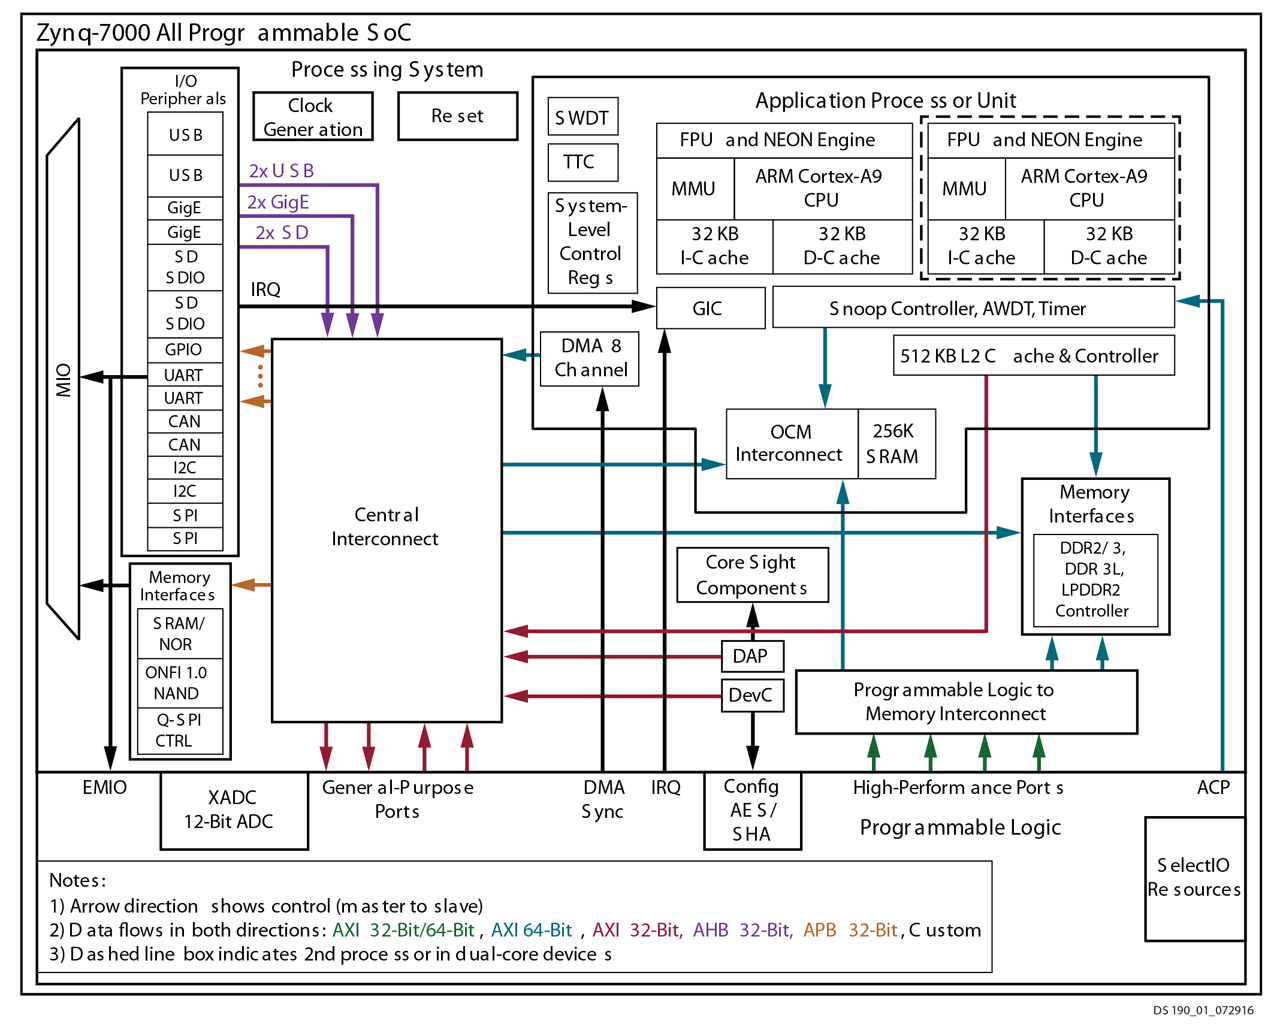
\includegraphics[width=1\textwidth]{images/Zynq-7000-Overview}
    \caption{Schemat ogólny architektury układu Zynq-7000.}
    \label{fig:zynq7000}
\end{figure}

\section{Interfejs AXI}
 AXI (ang. Advanced eXtensible Interface zawansowany rozszerzalny interfejs) jest częścią ARM AMBA (ang. Advanced Microcontroller Bus Architecture) – otwartego standardu, specyfikacją do zarządzania i połączeń między blokami funkcyjnymi w SoC. Aktualnie jest stosowana AMBA 4.0 która wprowadziła drugą wersję AXI, AXI4. Występują trzy typy interfejsów dla AXI4:
\begin{itemize}
\item AXI4 – stosowany w wysokowydajnych transferach w przestrzeni pamięci (ang. memory-mapped)
\item AXI4-Lite – stosowany dla prostszych operacji w przestrzeni pamięci (na przykład do komunikacji z rejestrami kontrolnymi i statusu)
\item AXI4-Stream – stosowany do wysokiej prędkości transmisji strumieniowych
\end{itemize}
Specyfikacja interfejsu zakłada komunikację pomiędzy pojedynczym AXI master i pojedynczym AXI slave, która ma na celu wymianę informacji pomiędzy tymi dwoma blokami funkcyjnymi IP core. Kilkanaście interfejsów AXI master i slave mogą zostać połączone między sobą za pomocą specjalnej struktury zwanej interconnect block (blok międzypołączeniowy) w której odbywa się trasowanie połączeń do poszczególnych bloków. 

AXI4 i AXI4-Lite składają się z 5 różnych kanałów:
\begin{itemize}
\item Kanał adresu odczytu,
\item Kanał adresu zapisu,
\item Kanał danych odczytanych
\item Kanał danych do zapisania
\item Kanał potwierdzenia zapisu
\end{itemize}
Dane mogą płynąć w obie strony pomiędzy master a slave jednocześnie. Ilość danych które można przesłać w jednej transakcji w przypadku AXI4 wynosi 256 transferów, zaś AXI4-Lite pozwala na tylko 1 transmisję.

AXI4-Stream nie posiada pola adresowego, a dane mogą być przesyłane nieprzerwanie. 
\section{Wykorzystanie AXI-Stream do transmisji sygnału video.} 
W odróżnieniu od klasycznej implementacji przetwarzania strumieniowego video, w AXI-Stream przesyłane są jedynie aktywne piksele. Linie synchronizacji poziomej i pionowej są odrzucane albo są połączane do specjalnego bloku detekcji timingów który mierzy parametry wchodzącego strumienia wizyjnego (ilość pikseli na linie, czas ilość aktywnych linii, czas wyciemnienia itd.). Podobnie informacje o synchronizacji są dodawane przez blok generujący timingi.

Do transmisji wykorzystane jest 6 linii: jedna linia danych i pięć kontrolno-sterujących. 
\begin{itemize}
\item Video Data – linia danych o szerokości jednego (albo dwóch) pikseli. Szerokość tej linii powinna być wielokrotnością liczby osim (16, 24, 48 itd.)
\item Valid – Linia podająca czy dane piksela są poprawne,
\item Ready – Linia kontrolna informująca urządzenie master że slave jest gotowy do transmisji danych,
\item Start Of Frame – linia która wskazuje pierwszy piksel nowej ramki,
\item End Of Line – linia wskazująca ostatni piksel w linii.
\end{itemize}
Aby mógł wystąpić poprawny transfer danych linie Valid i Ready muszą być w stanie wysokim podczas rosnącego zbocza zegara. Przykładowe nawiązanie transmisji przedstawia rysunek \ref{fig:handshake}

\begin{figure}[h]
    \centering
    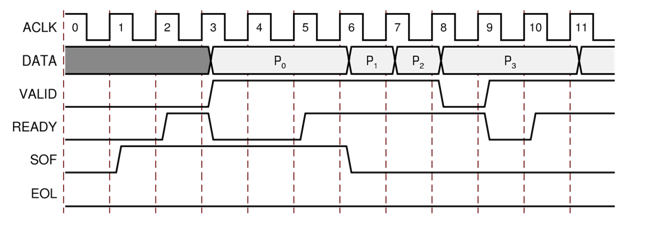
\includegraphics[width=1\textwidth]{images/axi-stream_hendshake}
    \caption{Przykład rozpoczęcia transmisji Reday/Valid.}
    \label{fig:handshake}
\end{figure}

\section{AXI VDMA}
Wiele aplikacji wizyjnych wymaga przechowania całej ramki obrazu w celu jej dalszej obróbki np. podczas skalowania, przycinania bądź dopasowania ilości klatek na sekundę. Część programowalna układu Zynq zazwyczaj nie posiada wystarczającej liczby zasobów do przechowanie klatki obrazu w swojej strukturze. W tym celu jest wykorzystywany mechanizm bezpośredniego dostępu do pamięci który pozwala na przesłanie i wczytanie danych z logiki programowalnej do pamięci RAM bez konieczności angażowania procesora. Realizuje się to poprzez IP-Core AXI VDMA. Zapewnia on przejście między interfejsem AXI4-Stream a AXI4 Memory Map w obu kierunkach. Przed rozpoczęciem przesyłania IP-Core jest konfigurowany poprzez interfejs AXI4-Lite. Konfiguracja zawiera adres w pamięci RAM do którego ma być zapisana bądź wczytana ramka obrazu. Po wgraniu do pamięci ramki kontroler może wywołać przerwanie dla systemu procesorowego.


\printbibliography

\end{document}
